\documentclass[a4paper,12pt]{article} 
\usepackage[margin=1in]{geometry}
\usepackage[utf8]{inputenc}
\usepackage[english]{babel}
\usepackage[shortlabels]{enumitem}
\usepackage{fancyhdr}
\usepackage{fancyvrb}
\usepackage{amssymb}
\usepackage{graphicx}
\usepackage{amsmath}
\usepackage{mathtools}
\usepackage{tikz}
\usepackage{float}
\usetikzlibrary{automata, arrows}
\usepackage{comment}
\usepackage{hyperref}
\usepackage{pdfpages}
\usepackage[toc,page]{appendix}
\usepackage[shortlabels]{enumitem}


\usepackage{algorithm}
\usepackage{caption}
\usepackage[noend]{algpseudocode}


\algnewcommand\algorithmicforeach{\textbf{for each}}
\algdef{S}[FOR]{ForEach}[1]{\algorithmicforeach\ #1\ \algorithmicdo}
%removes caption from alorithm caption
\captionsetup[algorithm]{labelformat=empty}




\hypersetup{colorlinks,urlcolor=blue}



\pagestyle{fancy}
\fancyhf{}
\rfoot{Page \thepage}


\begin{document}

\begin{titlepage}
   \begin{center}
       \vspace*{1cm}
 
       \textbf{CAB301 Algorithms and Complexity - Semester 1 2020}
 
       \vspace{0.5cm}
        \LARGE{Development of a Software Application for a Community Library to Manage its Movie DVDs}
 
       \vspace{1.5cm}

       \vfill
       
       \vspace{0.8cm}
       \normalsize
 	   Written in \LaTeX \\
       
\includegraphics[width=0.4\textwidth]{QUT}

       \large
       \textbf{Jake Burrell}\\
       \textbf{n9712291}

       \vspace{1.5cm}
 
       \normalsize
 	   Bachelor of Information Technology\\
       Science and Engineering Faculty\\
       Queensland University of Technology\\
       Australia\\ 
   \end{center}
\end{titlepage}

\section{Top 10 most frequently borrowed movie algorithm}


\begin{algorithm}
\caption{\textbf{Return top 10 Movies($ \mathcal B[m(root)]$)}}
\emph{//Uses a generic BinarySearchTree class I created}\\
\emph{//This class is iterable using in-order traversal}\\
\emph{//Uses a MoviePair class to store name of movie and number of borrows}\\
\emph{//MoviePair comparable such that MoviePair objects with more borrows are seen as}\\
\emph{//being less than those with less borrows}\\
\emph{//Input: A Binary Search Tree of Movies}\\
\emph{//Output: An array of movie names associated with the top ten movies}
\begin{algorithmic}[1]
\State $\mathcal T[mp] \leftarrow \phi$ \emph{//Initialized BST of MoviePair with root null}
\State $A[0..9] \leftarrow \phi$ \emph{//Initializes empty array of 10 items}
\ForEach {$m \in \mathcal B $} \emph{//For each movie in the BST}
	\State $mp \leftarrow m[m.name, m.borrows]$ 
	\State $ \mathcal T[mp].addNode(mp)$
\EndFor
\State $i = 0$
\ForEach {$mp \in \mathcal T[mp]$}
	\If {$i = 10$}
		\State $break$
	\EndIf
	\State $A[i] = mp.name$
	\State $i \leftarrow i + 1$
\EndFor
\State \textbf{return} $A[1..9]$
\end{algorithmic}
\end{algorithm}
\section{Analysis of the Top 10 Algorithm}
In examining the first for loop the either operation $mp \leftarrow m[m.name, m.borrows]$ or $ \mathcal T[mp].addNode(mp)$ could be consider the basic operations. These basic operations are in a for loop which iterates over each node in the input Binary Search Tree. Since the number of movies in the BST equates to the input size $n$ then the time complexity of the first for loop could be consider $c(n) = n$. Now since the second for loop contains a break within it that breaks after 10 iterations. Its complexity can therefore be considered a constant and does not need to be considered. Thus leaving the efficiency as $c(n) = n$ and the asymptotic efficiency class as $c(n) = \Theta(n)$.

\newpage

\section{Demonstration of the Community Library Movie Management Software}

\begin{figure}[!htb]
\centering
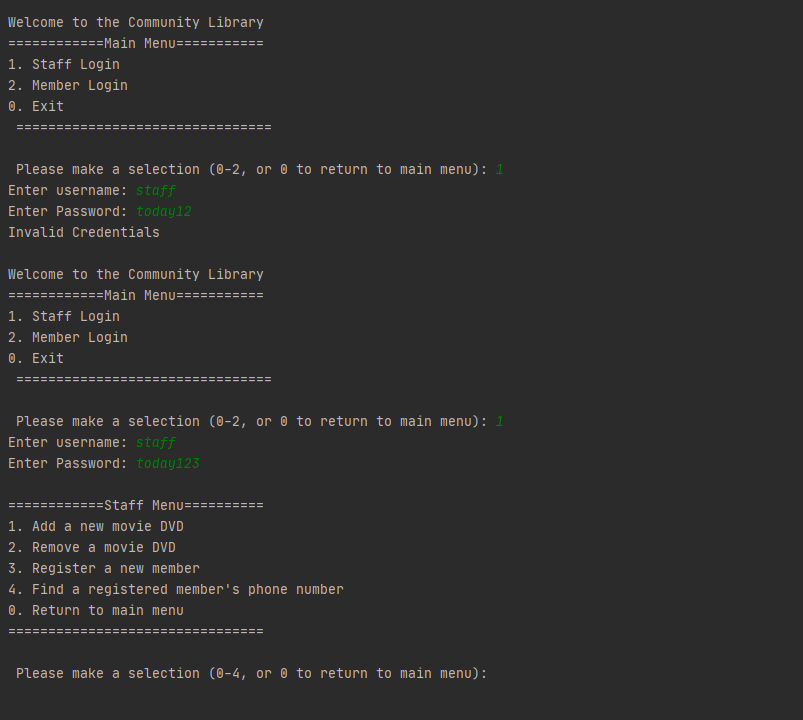
\includegraphics[width=1\textwidth]{1}
\caption{Logging in as a staff member}
\medskip
\small
As can be seen when logging in with invalid credentials the access is refused. When logging in with the valid staff credentials the user is returned the staff menu
\end{figure}

\begin{figure}[!htb]
\centering
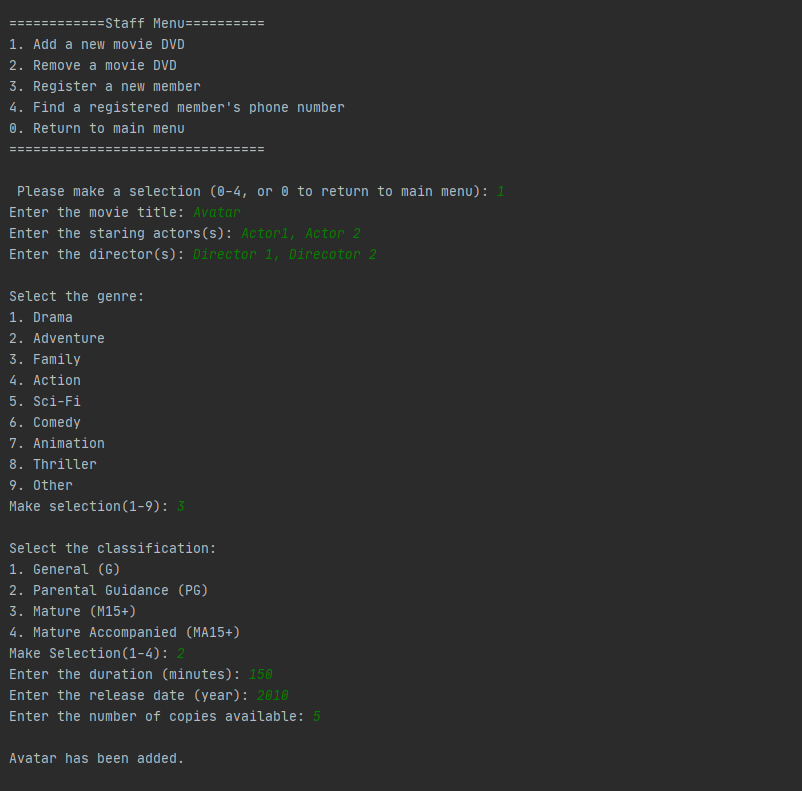
\includegraphics[width=1\textwidth]{2}
\caption{Staff creating a new movie}
\medskip
\small
The user can then selects 1 in order to add a new movie. They are then presented with a series of prompts in order to select the movie attributes. These include the movie title, list of directors, a list of actors, the genre, classification, duration, release date and available copies 
\end{figure}

\begin{figure}[!htb]
\centering
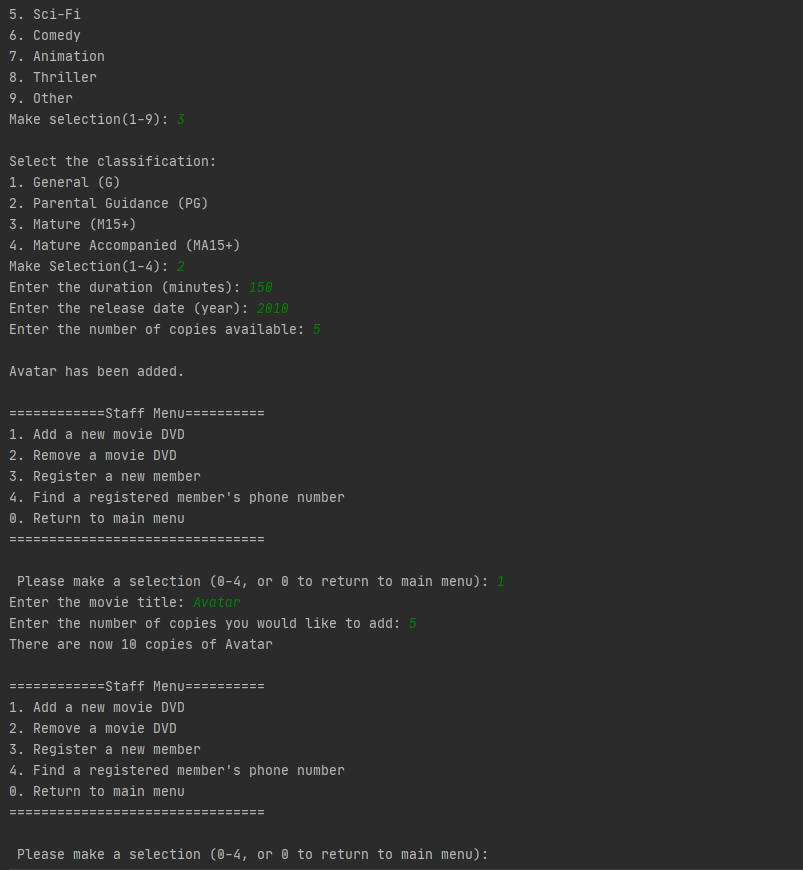
\includegraphics[width=1\textwidth]{3}
\caption{Adding copies to the movie}
\medskip
\small
If the user re-enters the number 1 once returned back to the staff menu and then enters an existing movie. As can be seen they can add additional copies of the movie.
\end{figure}

\begin{figure}[!htb]
\centering
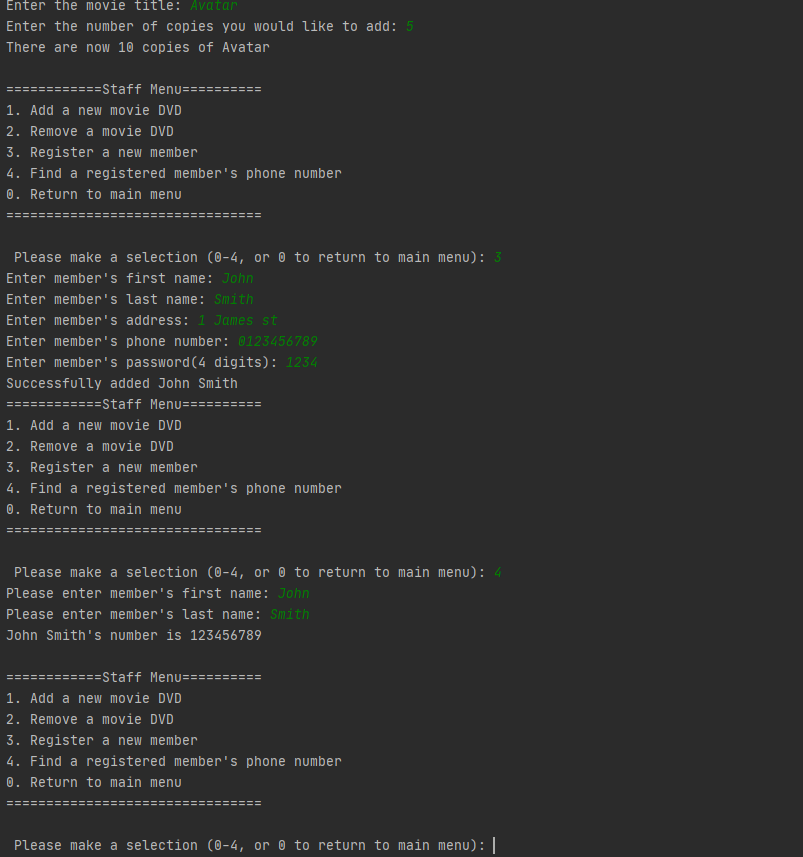
\includegraphics[width=1\textwidth]{4}
\caption{Creating a New User and Searching for their number}
\medskip
\small
From the staff menu the user can also add a user by entering 3. They are then prompted to enter the following details about the user: first name, last name, address, number, and a four digit password. As seen above once the user is created their number can also be retrieved.
\end{figure}

\begin{figure}[!htb]
\centering
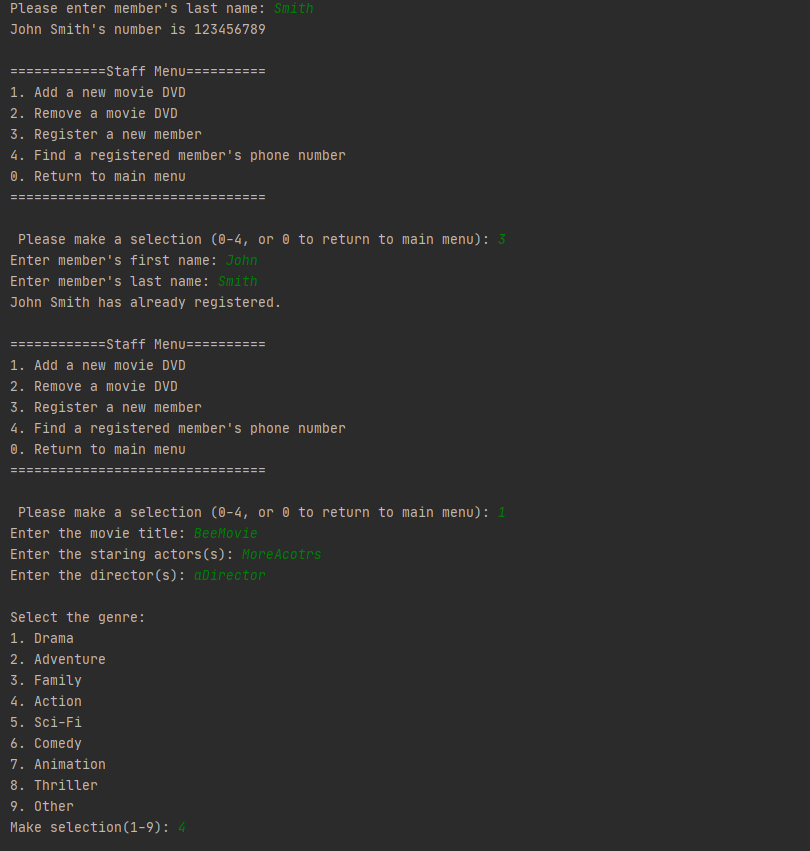
\includegraphics[width=1\textwidth]{5}
\caption{Registering a user a second time}
\medskip
\small
As can be seen, a user of the same name cannot be added to the system twice. After which two a couple more movie where create for demonstration
\end{figure}


\begin{figure}[!htb]
\centering
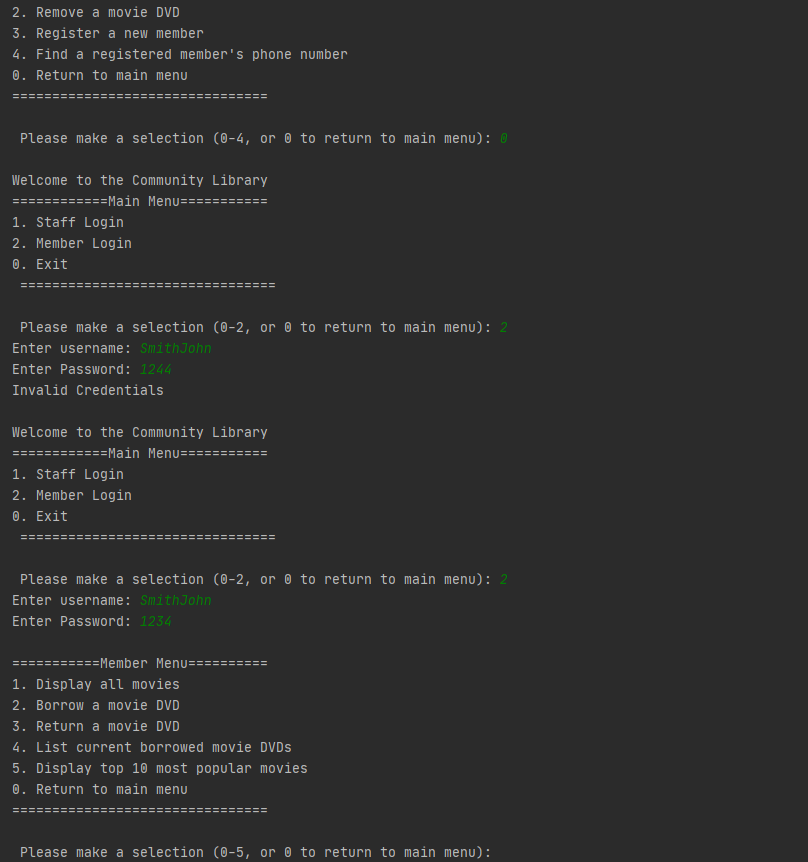
\includegraphics[width=1\textwidth]{6}
\caption{Logging in as a member}
\medskip
\small
Using 0 to return to the main menu a user can then log in with as an existing staff menu provided the correct password is provided.
\end{figure}

\begin{figure}[!htb]
\centering
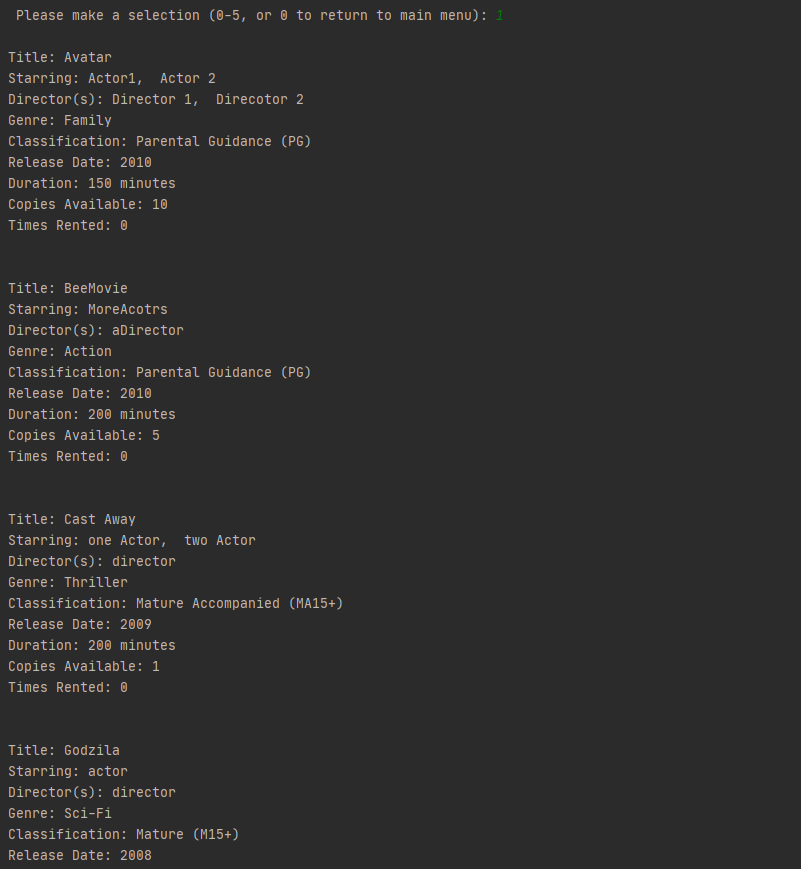
\includegraphics[width=1\textwidth]{7}
\caption{Displaying Movies Alphabetically}
\medskip
\small
From the member menu a user can display movies by entering the number 1. As can be see each movie is displayed with all its information and in alphabetical order
\end{figure}

\begin{figure}[!htb]
\centering
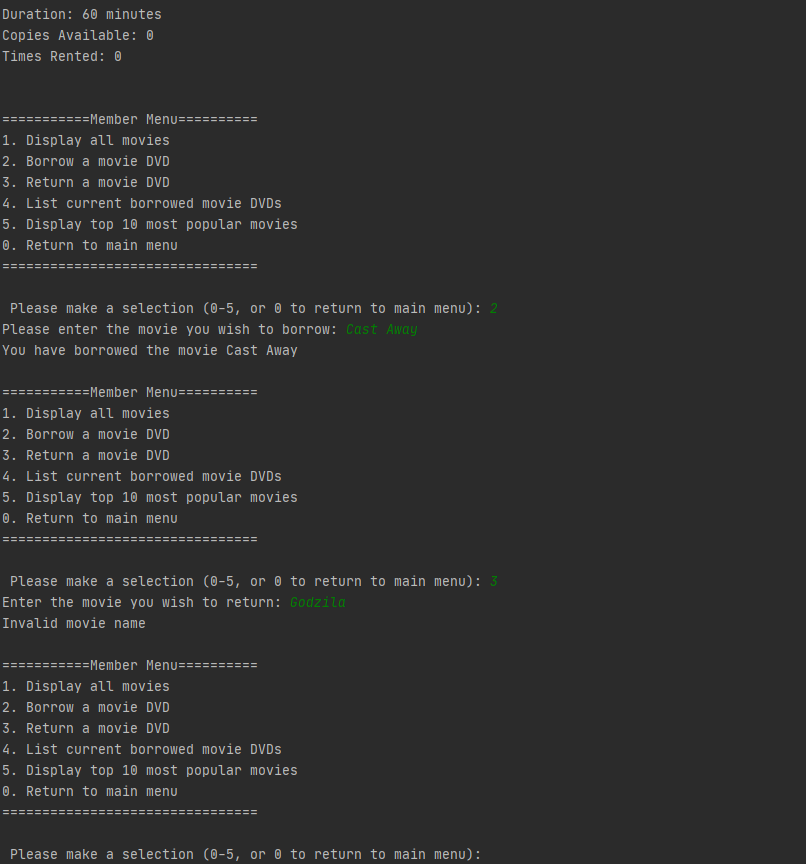
\includegraphics[width=1\textwidth]{8}
\caption{Borrowing a movie}
\medskip
\small
Once back a the staff menu that the user is returned to they can select 2 and enter the name of the movie they wish to borrow. Notice if the movie is a movie that has no copies available, such as Godzilla. The user is unable to borrow it.
\end{figure}

\begin{figure}[!htb]
\centering
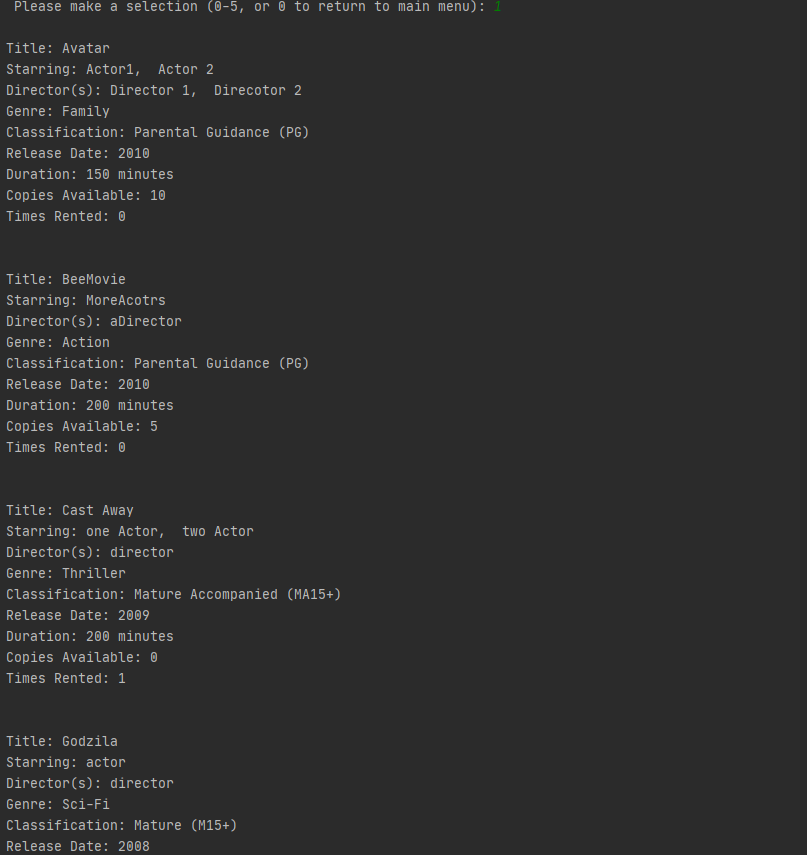
\includegraphics[width=1\textwidth]{9}
\caption{Times rented incremented and copies available is decremented}
\medskip
\small
Now notice that since Cast Away has now been borrowed their are now no longer any copies available. Also since it was rented its now been recorded that its been rented once.
\end{figure}

\begin{figure}[!htb]
\centering
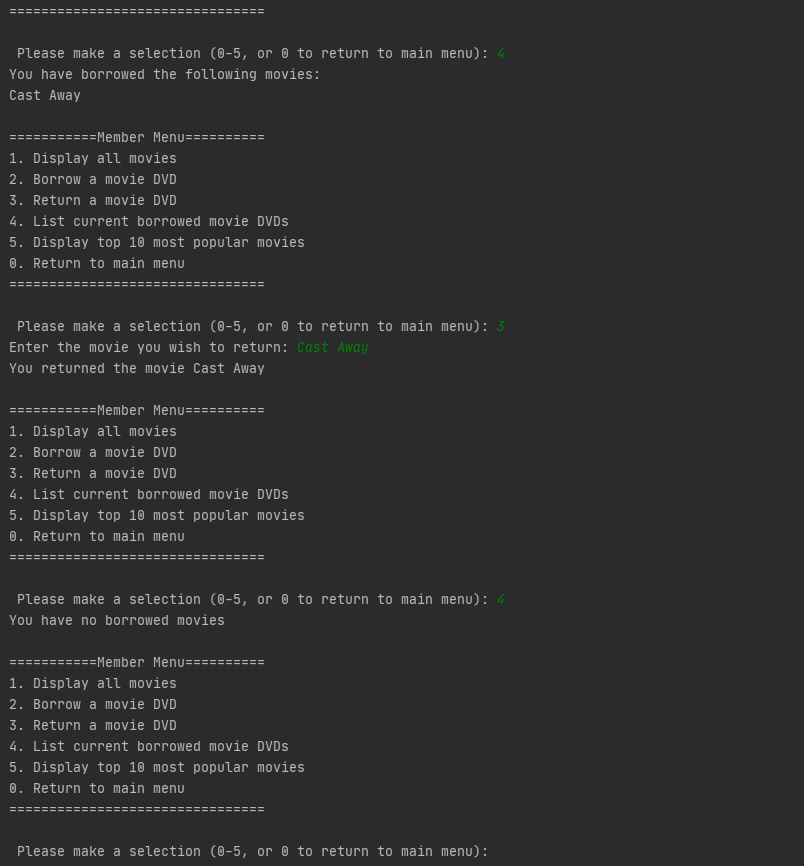
\includegraphics[width=1\textwidth]{10}
\caption{Listing borrowed movies}
\medskip
\small
From the member menu it can be seen above that by entering 4 the member can view their borrowed movies. Notice that it lists the movie Cast Away then after returning the movie using 3 and entering the name again. It now states that they have no borrowed movies 
\end{figure}

\begin{figure}[!htb]
\centering
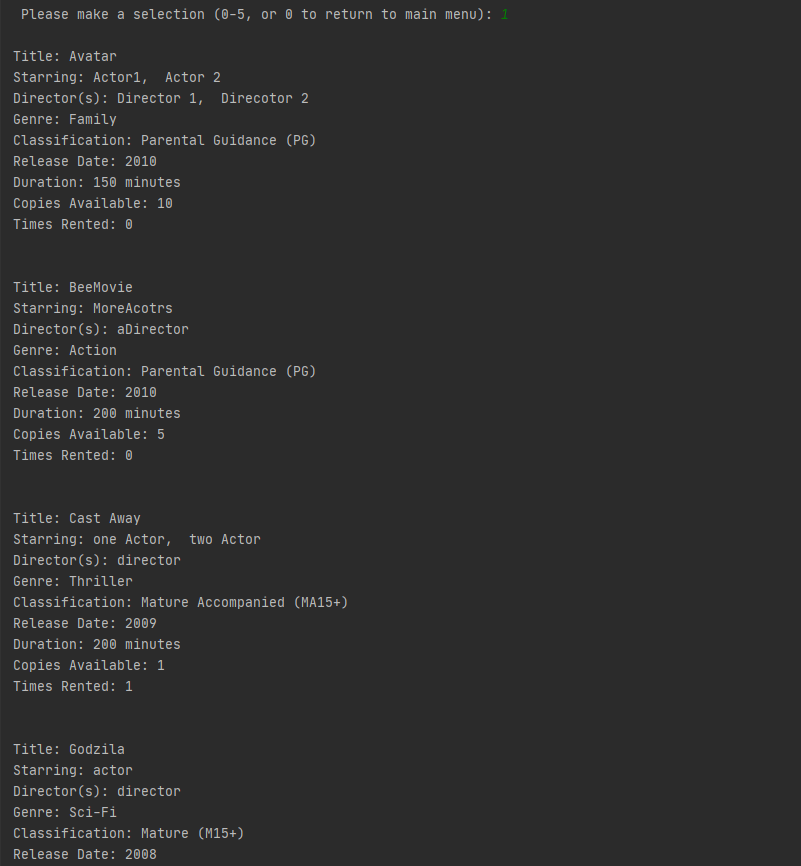
\includegraphics[width=1\textwidth]{11}
\caption{Copies incremented again once movie returned}
\medskip
\small
Notice now that the movie Cast Away now has copies available since its been returned
\end{figure}


\begin{figure}[!htb]
\centering
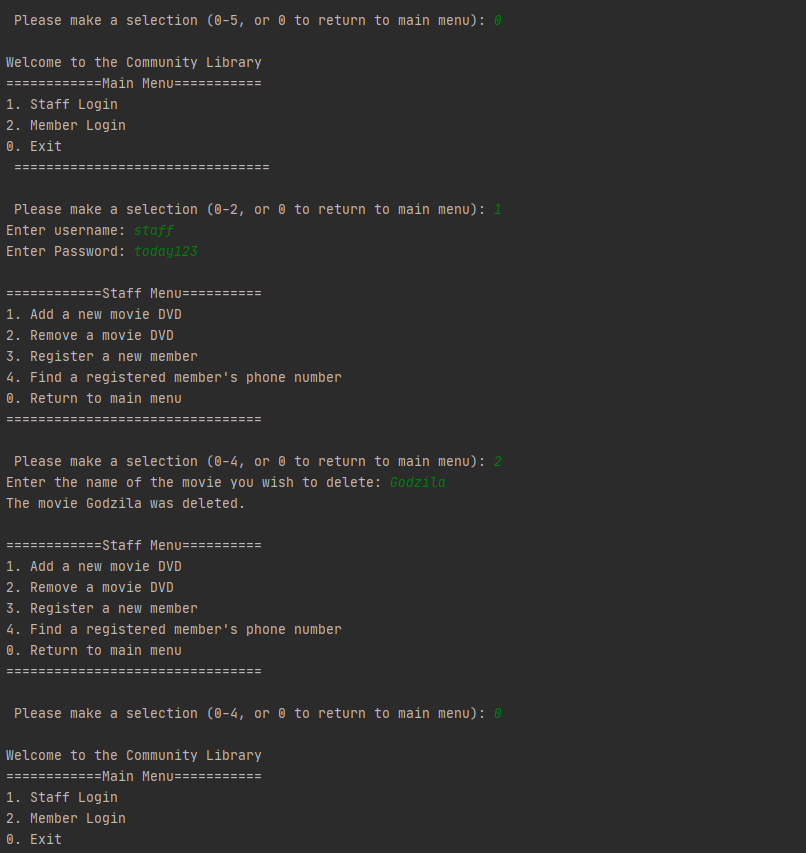
\includegraphics[width=1\textwidth]{12}
\caption{Deleting Movie}
\medskip
\small
As seen above, entering zero returns the user to the main menu. Now a staff member logs in and by selecting 2 they are able to remove a movie Godzila
\end{figure}

\begin{figure}[!htb]
\centering
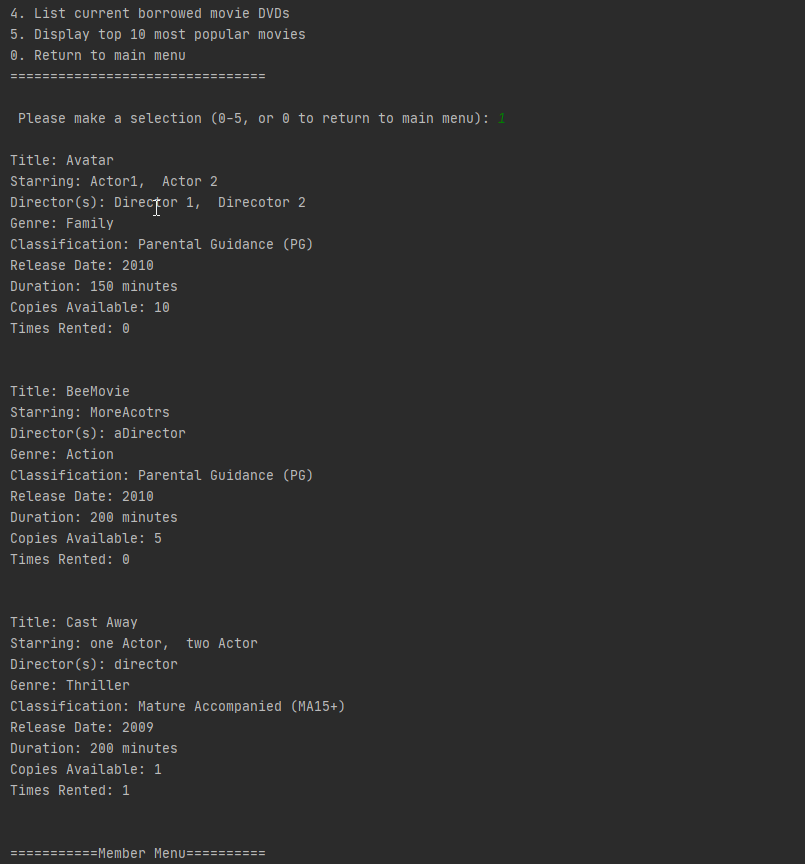
\includegraphics[width=1\textwidth]{13}
\caption{Movie deleted}
\medskip
\small
Now returning to the main menu, then logging in as a member again and displaying movies. It can be seen that the movie Godzila is gone
\end{figure}




\end{document}
\begin{figure}[!htb]
\centering
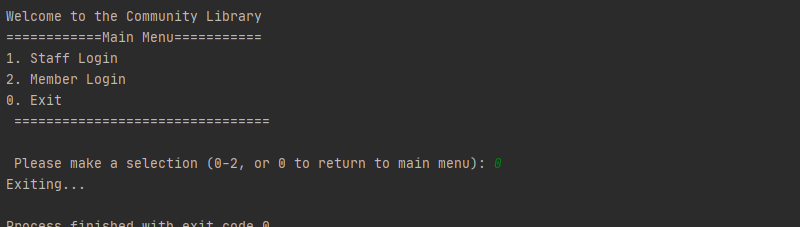
\includegraphics[width=1\textwidth]{14}
\caption{Exiting}
\medskip
\small
Now returning to the main menu again exiting the program by selecting 0 can be seen
\end{figure}
